\section{Introduction}
\begin{frame}{\VideoName}
    \tableofcontents[currentsection]
\end{frame}

\begin{frame}{Countermeasures}
    \begin{itemize}
        \item Protocol level: design cryptographic protocols to survive leakage analysis
        \begin{itemize}
            \item Limiting the number of communications that can be performed with any given key, fewer measurements can be done by the attacker for the same key
            \item Re-keying\footnote{Medwed, M., Standaert, F. X., Großschädl, J., \& Regazzoni, F. (2010, May). Fresh re-keying: Security against side-channel and fault attacks for low-cost devices. In International Conference on Cryptology in Africa (pp. 279-296). Springer, Berlin, Heidelberg.}
        \end{itemize}
         \item Cryptographic primitive level
        \begin{itemize}
            \item Proposal of new cipher design
        \end{itemize}
    \end{itemize}
\end{frame}

\begin{frame}{Countermeasures}
    \begin{itemize}
        \item Implementation level
        \begin{itemize}
            \item Time randomization\footnote{May, D., Muller, H. L., \& Smart, N. P. (2001, May). Random register renaming to foil DPA. In International Workshop on Cryptographic Hardware and Embedded Systems (pp. 28-38). Springer, Berlin, Heidelberg.}
            \item Encryption of the buses\footnote{Brier, E., Handschuh, H., \& Tymen, C. (2001, May). Fast primitives for internal data scrambling in tamper resistant hardware. In International Workshop on Cryptographic Hardware and Embedded Systems (pp. 16-27). Springer, Berlin, Heidelberg.}
            \item \textcolor{blue}{Hiding}
            \item \textcolor{blue}{Masking and blinding}
        \end{itemize}
    \end{itemize}
\end{frame}

\begin{frame}{Countermeasures}
    \begin{itemize}
        \item Architecture level
        \begin{itemize}
            \item Use non-deterministic processor to randomly change the sequence of the executed program during each execution\footnote{May, D., Muller, H. L., \& Smart, N. P. (2001, July). Non-deterministic processors. In Australasian Conference on Information Security and Privacy (pp. 115-129). Springer, Berlin, Heidelberg.} 
            \item Integrate secure instructions into a non-secure processor\footnote{Saputra, H., Vijaykrishnan, N., Kandemir, M., Irwin, M. J., \& Brooks, R. (2003). Masking the energy behaviour of encryption algorithms. IEE Proceedings-Computers and Digital Techniques, 150(5), 274-284.}
        \end{itemize}  
    \end{itemize}
\end{frame}

\begin{frame}{Countermeasures}
    \begin{itemize}
        \item Hardware level
        \begin{itemize}
            \item Conforming glues\footnote{Anderson, R., \& Kuhn, M. (1996, November). Tamper resistance -- a cautionary note. In Proceedings of the second Usenix workshop on electronic commerce (Vol. 2, pp. 1-11).}
            \item Protective coating\footnote{Tuyls, P., Schrijen, G. J., Škorić, B., Geloven, J. V., Verhaegh, N., \& Wolters, R. (2006, October). Read-proof hardware from protective coatings. In International Workshop on Cryptographic Hardware and Embedded Systems (pp. 369-383). Springer, Berlin, Heidelberg.}
            \item Detachable power supplies\footnote{Shamir, A. (2000, August). Protecting smart cards from passive power analysis with detached power supplies. In International Workshop on Cryptographic Hardware and Embedded Systems (pp. 71-77). Springer, Berlin, Heidelberg.}
        \end{itemize} 
    \end{itemize}
\end{frame}

\begin{frame}{Hiding and masking/blinding}
\begin{itemize}
    \item We have seen how the dependency of a device's leakages (power consumption) on data and operations can be exploited to recover the secret keys of a cryptographic implementation.
   \item Goal: make the leakage of the DUT independent of the operations or the intermediate values of the executed cryptographic implementation.
    \item Hiding -- remove the operation/data dependency of leakage
    \begin{itemize}
        \item Change the leakage of the DUT in a way that every operation requires a similar (balance leakages) or a random (randomize leakages) amount of energy.
    \end{itemize}
    \item Masking/blinding -- remove the data dependency of leakage by randomizing the intermediate values that the DUT is processing
    \begin{itemize}
        \item The rationale is that since the value being processed in the DUT is randomized and independent of the intermediate value of the cryptographic computation, we cannot capture information on the actual intermediate value from the leakages.
        \item Symmetric block cipher: masking
        \item Asymmetric cipher: blinding
    \end{itemize}
\end{itemize}    
\end{frame}


\begin{frame}{Hiding -- randomizing power consumption}
    \begin{itemize}
       \item Insert random delay (jitter)\footnote{Coron, J. S., \& Kizhvatov, I. (2009, September). An efficient method for random delay generation in embedded software. In International Workshop on Cryptographic Hardware and Embedded Systems (pp. 156-170). Springer, Berlin, Heidelberg.}
       \item Shuffle the execution order of independent operations
       \begin{itemize}
           \item Sboxes in AES\footnote{Herbst, C., Oswald, E., \& Mangard, S. (2006, June). An AES smart card implementation resistant to power analysis attacks. In International conference on applied cryptography and network security. Springer.}
           \item Randomize the sequence of square and multiply\footnote{Walter, C. D. (2002, February). MIST: An efficient, randomized exponentiation algorithm for resisting power analysis. In Cryptographers’ Track at the RSA Conference. Springer.}
       \end{itemize}
       \item Using residue number systems allow randomizing the representation of finite field elements for computing exponentiation\footnote{Bajard, J. C., Imbert, L., Liardet, P. Y., \& Teglia, Y. (2004, August). Leak resistant arithmetic. In International Workshop on Cryptographic Hardware and Embedded Systems. Springer.}
    \end{itemize}
\end{frame}

\begin{frame}{Hiding -- balancing power consumption}
    \begin{itemize}
        \item Cell level, logic designs
        \begin{itemize}
            \item Dual-rail precharge logic (DPL)\footnote{Tiri, K., \& Verbauwhede, I. (2006). A digital design flow for secure integrated circuits. IEEE Transactions on Computer-Aided Design of Integrated Circuits and Systems, 25(7), 1197-1208.}, in pre-charge phase, values in the weries are set to a precharge value (either $0$ or $1$), during evaluation phase, one wire carries the signal $0$ and the other wire carries the signal $1$
            \begin{itemize}
                \item Using code $\{01,10\}$ for encoding $0,1$
            \end{itemize}
            \item Dynamic and differential logic styles \footnote{Tiri, K., Akmal, M., \& Verbauwhede, I. (2002, September). A dynamic and differential CMOS logic with signal independent power consumption to withstand differential power analysis on smart cards. In Proceedings of the 28th European solid-state circuits conference (pp. 403-406). IEEE.}
        \end{itemize}
    \end{itemize}
\end{frame}

%%
\begin{frame}{Hiding -- balancing power consumption}
\begin{itemize}
    \item Software level
        \begin{itemize}
            \item DPL in software for symmetric block ciphers\footnote{Hoogvorst, P., Duc, G., \& Danger, J. L. (2011). Software implementation of dual-rail representation. COSADE, 51, 24-25.}
            \item DPL in software with proved security for bitsliced implementation of PRESENT\footnote{Rauzy, P., Guilley, S., \& Najm, Z. (2013). Formally Proved Security of Assembly Code Against Leakage. IACR Cryptol. ePrint Arch., 2013, 554.}
            \item Linear complementary dual code\footnote{Carlet, C., \& Guilley, S. (2015). Complementary dual codes for counter-measures to side-channel attacks. In Coding Theory and Applications (pp. 97-105). Springer, Cham.}
            \item Error detecting and correcting code in software\footnote{Breier, J., \& Hou, X. (2017, February). Feeding two cats with one bowl: On designing a fault and side-channel resistant software encoding scheme. In Cryptographers’ Track at the RSA Conference (pp. 77-94). Springer, Cham.}
            \item \textcolor{blue}{Square and multiply-always for computing exponentiation in RSA}\footnote{Coron, J. S. (1999, August). Resistance against differential power analysis for elliptic curve cryptosystems. In International workshop on cryptographic hardware and embedded systems (pp. 292-302). Springer, Berlin, Heidelberg.}
        \end{itemize}
\end{itemize}
\end{frame}

\begin{frame}{Masking and blinding}
    \begin{itemize}
        \item Let $\boldsymbol{v}$ be the secret intermediate value that we would like to mask.
      \item The masked value, denoted $\boldsymbol{v}_{\m}$, concealed by a random value $\m$, called a \textit{mask}, with a binary operation $\cdot$ such that
\[
\boldsymbol{v}_{\m}=\boldsymbol{v}\cdot\m.
\]
    \end{itemize}
\end{frame}

\begin{frame}{Masking}
    \begin{itemize}
        \item \textcolor{blue}{Boolean masking, the binary operation is bitwise \texttt{XOR}}
        \item Arithmetic masking, the binary operation is modular addition or modular multiplication
        \item Affine masking\footnote{Willich, M. V. (2001, December). A technique with an information-theoretic basis for protecting secret data from differential power attacks. In IMA International Conference on Cryptography and Coding (pp. 44-62). Springer, Berlin, Heidelberg.}
        \item Polynomial masking\footnote{Goubin, L., \& Martinelli, A. (2011, September). Protecting AES with Shamir’s secret sharing scheme. In International Workshop on Cryptographic Hardware and Embedded Systems (pp. 79-94). Springer, Berlin, Heidelberg.}
        \item Inner product masking\footnote{Balasch, J., Faust, S., Gierlichs, B., \& Verbauwhede, I. (2012, December). Theory and practice of a leakage resilient masking scheme. In International Conference on the Theory and Application of Cryptology and Information Security (pp. 758-775). Springer, Berlin, Heidelberg.}
    \end{itemize}
\end{frame}

\begin{frame}{Masking -- more methods in hardware implementations}
    \begin{itemize}
        \item Masking buses\footnote{Benini, L., Galati, A., Macii, A., Macii, E., \& Poncino, M. (2003, August). Energy-efficient data scrambling on memory-processor interfaces. In Proceedings of the 2003 International Symposium on Low Power Electronics and Design, 2003. ISLPED'03. (pp. 26-29). IEEE.}
        \item Boolean masking with DLP\footnote{Popp, T., \& Mangard, S. (2005, August). Masked dual-rail pre-charge logic: DPA-resistance without routing constraints. In International Workshop on Cryptographic Hardware and Embedded Systems (pp. 172-186). Springer, Berlin, Heidelberg.}
        \item Random precharging\footnote{Bucci, M., Guglielmo, M., Luzzi, R., \& Trifiletti, A. (2004, September). A power consumption randomization countermeasure for DPA-resistant cryptographic processors. In International Workshop on Power and Timing Modeling, Optimization and Simulation (pp. 481-490). Springer, Berlin, Heidelberg.}
    \end{itemize}
\end{frame}

\section{Masking for PRESENT}
\begin{frame}{\VideoName}
    \tableofcontents[currentsection]
\end{frame}

\begin{frame}{Boolean masking}
    \begin{itemize}
        \item Proven to be secure given that the source of randomness is truly random\footnote{Prouff, E., \& Rivain, M. (2013, May). Masking against side-channel attacks: A formal security proof. In Annual International Conference on the Theory and Applications of Cryptographic Techniques (pp. 142-159). Springer, Berlin, Heidelberg.}
        \item The cryptographic algorithm needs to be changed a bit for us to carry out computations with the masked intermediate values and keep track of all the masks
        \item At the end of the encryption, we can remove the masks to output the original ciphertext
    \end{itemize}
\end{frame}

\begin{frame}{Masking scheme}
    \begin{itemize}
        \item A \textit{masking scheme} specifies how masks are applied to the plaintext and intermediate values, as well as how they are removed from the ciphertext.
        \item There are a few principles we follow for a masking scheme design
        \begin{itemize}
             \item All intermediate values should be masked during the computation.
     In particular, we would apply masks to the plaintext (and the key).
    \item We assume the attacker does not have knowledge of the masks -- otherwise, the attacker can carry out a DPA attack by making hypotheses about the key values.
    \item When some intermediate values are to be \texttt{XOR}-ed with each other (e.g. in AES MixClomns operation), different masks should be applied to each of them.
    \item Each encryption has a different set of randomly generated masks.
        \end{itemize}
        \item For any function $f$, the mask that is applied to an input of $f$ is called the \textit{input mask} of $f$.
        \item The corresponding mask for the output is called the \textit{output mask} for $f$.
    \end{itemize}
\end{frame}


\begin{frame}{Linear function}
    \begin{definition}
    Let $f:\FF_2^{m_1}\to\FF_2^{m_2}$ be a function, where $m_1$ and $m_2$ are positive integers.
$f$ is said to be \textit{linear} (w.r.t. $\oplus$) if for any $\boldsymbol{x},\boldsymbol{y}\in\FF_2^{m_1}$, we have
\[
    f(\boldsymbol{x}\oplus\boldsymbol{y})=f(\boldsymbol{x})\oplus f(\boldsymbol{y}).
\]
$f$ is \textit{non-linear} if it is not linear.
\end{definition}
\begin{example}
    \begin{itemize}
        \item AddRoundKey operation in AES round function is a linear function. In fact, bitwise \texttt{XOR} with a round key is a linear function in general.
        \item DES Sboxes are non-linear functions.
        Any Sbox proposed so far for symmetric block ciphers is non-linear.
        \item pLayer in PRESENT round function is linear.
        % \item MixColumns operation in AES is linear.
    \end{itemize}
\end{example}
\end{frame}

\begin{frame}{Boolean masking for linear functions}
    \begin{itemize}
        \item With Boolean masking, it is easy to keep track of the masks with linear operations.
       \item Let $f$ be a linear operation and take any input of $f$, $\boldsymbol{v}$, with a corresponding mask $\m$, we have
\[
f(\boldsymbol{v}\oplus\m)=f(\boldsymbol{v})\oplus f(\m).
\]
\item When the input mask is $\m$, the output mask is given by $f(\m)$.
\item One of the main challenges in designing a masking scheme is to find ways to keep track of masks for non-linear operations.
    \end{itemize}
\end{frame}


\begin{frame}{PRESENT -- encryption}
\begin{columns}[T] % align columns
\begin{column}{.55\textwidth}
\begin{itemize}
    \item Block length: $64$
       \item Number of rounds: $31$
       \item Key length: $80$ or $128$.
    \item Round function: addRoundKey, sBoxLayer, and pLayer.
    \item After $31$ rounds, addRoundKey is applied again before the ciphertext output 
\end{itemize}
\begin{alertblock}{Remark}
    For PRESENT specification, we consider the $0$th bit of a value as the rightmost bit in its binary representation.
For example, the $0$th bit of $3=011_2$ is $1$, the $1$st bit is $1$ and the $2$nd bit is $0$.
\end{alertblock}
\end{column}%
\hfill%
\begin{column}{.5\textwidth}
\begin{figure}
    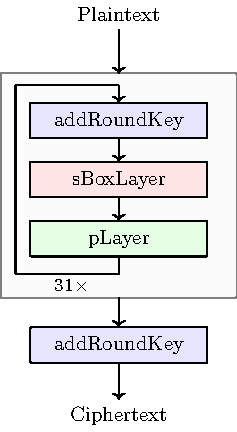
\includegraphics[width=0.6\textwidth]{fig/PRESENT.pdf}
\end{figure}
\end{column}%
\end{columns}
\end{frame}

\begin{frame}{PRESENT -- sBoxLayer}
    \begin{itemize}
        \item sBoxLayer applies sixteen $4-$bit Sboxes to each nibble of the current cipher state.
        \item For example, if the input is \texttt{0}, the output is \texttt{C}.
\begin{table}[htb]
\centering
\ttfamily
\begin{tabular}{cccccccccccccccc}\hline
 0 & 1 & 2 & 3 & 4 & 5 & 6 & 7 & 8 & 9 & A & B & C & D & E & F \\\hline
 C & 5 & 6 & B & 9 & 0 & A & D & 3 & E & F & 8 & 4 & 7 & 1 & 2\\\hline
\end{tabular}
\end{table}
    \end{itemize}
\begin{figure}
    \centering
    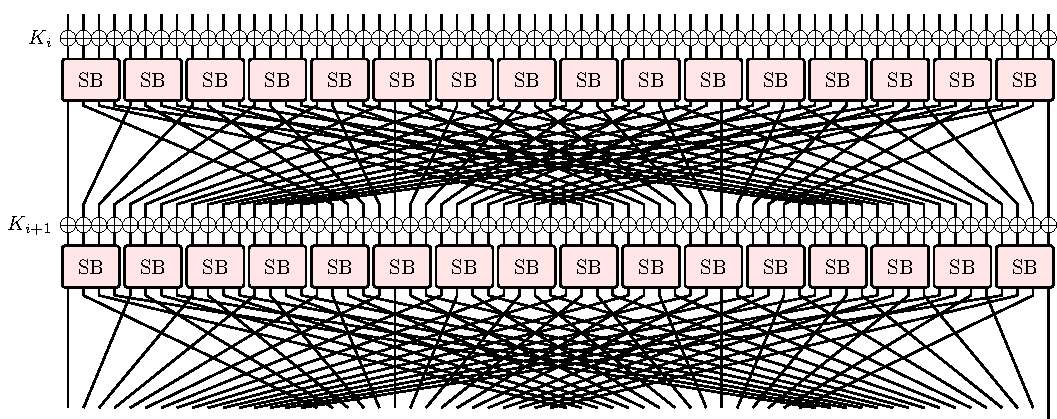
\includegraphics[width=0.9\textwidth]{fig/PRESENT_two_rounds.pdf}
\end{figure}
\end{frame}


\begin{frame}{PRESENT -- pLayer}
pLayer permutes the $64$ bits using the following formula:
\[
\text{pLayer}(j)=\left\lfloor\frac{j}{4}\right\rfloor+(j\mo 4)\times16,
\]
where $j$ denotes the bit position.
\begin{table}[htb]
\centering
\begin{tabular}{cccccccccccccccc}\hline
0 & 1 & 2 & 3 & 4 & 5 & 6 & 7 & 8 & 9 & 10 & 11 & 12 & 13 & 14 & 15 \\
0 & 16 & 32 & 48 & 1 & 17 & 33 & 49 & 2 & 18 & 34 & 50 & 3 & 19 & 35 & 51 \\\hline
16 & 17 & 18 & 19 & 20 & 21 & 22 & 23 & 24 & 25 & 26 & 27 & 28 & 29 & 30 & 31 \\
4 & 20 & 36 & 52 & 5 & 21 & 37 & 53 & 6 & 22 & 38 & 54 & 7 & 23 & 39 & 55 \\\hline
32 & 33 & 34 & 35 & 36 & 37 & 38 & 39 & 40 & 41 & 42 & 43 & 44 & 45 & 46 & 47 \\
8 & 24 & 40 & 56 & 9 & 25 & 41 & 57 & 10 & 26 & 42 & 58 & 11 & 27 & 43 & 59 \\\hline
48 & 49 & 50 & 51 & 52 & 53 & 54 & 55 & 56 & 57 & 58 & 59 & 60 & 61 & 62 & 63 \\
12 & 28 & 44 & 60 & 13 & 29 & 45 & 61 & 14 & 30 & 46 & 62 & 15 & 31 & 47 & 63\\\hline
\end{tabular}
\end{table}
\end{frame}

\begin{frame}{Masking PRESENT Sbox}
    \begin{itemize}
        \item Compute a lookup table T1 such that for any $\boldsymbol{v}\in\FF_2^4$, any input mask $\m_{\text{in}}$ and its corresponding output mask $\m_{\text{out}}$ for PRESENT Sbox,
\begin{equation*}
    \text{T1}[\boldsymbol{v}\oplus\m_{\text{in}},\m_{\text{in}}]=\text{SB}(\boldsymbol{v})\oplus\m_{\text{out}}.
\end{equation*}
\item Table T2 helps us keep track of the masks
\begin{equation*}
    \text{T2}[\m_{\text{in}}]=\m_{\text{out}},\quad\m_{\text{in}}=\texttt{0},\texttt{1},\dots,\texttt{F}.
\end{equation*}
\item Advantage: do not need to generate a masked Sbox lookup table whenever the input mask for the Sbox changes.
\item The size of T1 is $8\times4$, and the storage required is $2^8\times2^4=2^{12}$ bits, or $2^9$ bytes.
\item The table T2 requires $16$ bits of memory.
    \end{itemize}
\end{frame}

\begin{frame}{Masked cipher state}
    \begin{itemize}
        \item Since the pLayer operation is linear, we can simply apply pLayer to the masks to keep track of their changes.
\item We represent the intermediate values of PRESENT encryption as 
\begin{equation*}
    \boldsymbol{b}_{15},\boldsymbol{b}_{14},\dots,\boldsymbol{b}_1,\boldsymbol{b}_0,
\end{equation*}
where each $\boldsymbol{b}_j$ denotes a nibble of the cipher state.
\item At the beginning of one encryption, we randomly generate $16$ masks, and each is applied to one nibble of the plaintext.
\item Suppose the cipher state at the input of round $i$ is of the following format:
\[
\boldsymbol{b}_{15}\oplus\m^{i-1}_{15,\text{in}},\boldsymbol{b}_{14}\oplus\m^{i-1}_{14,\text{in}},\dots,\boldsymbol{b}_1\oplus\m^{i-1}_{1,\text{in}},\boldsymbol{b}_0\oplus\m^{i-1}_{0,\text{in}}.
\]
    \end{itemize}
\end{frame}


\begin{frame}{Masked addRoundKey}
Suppose the cipher state at the input of round $i$ is of the following format:
\[
\boldsymbol{b}_{15}\oplus\m^{i-1}_{15,\text{in}},\boldsymbol{b}_{14}\oplus\m^{i-1}_{14,\text{in}},\dots,\boldsymbol{b}_1\oplus\m^{i-1}_{1,\text{in}},\boldsymbol{b}_0\oplus\m^{i-1}_{0,\text{in}}.
\]
    \begin{itemize}
        \item We do not apply masks to the round keys. 
    Consequently, after the addRoundKey operation, each nibble of the cipher state still has the same mask
\[
\boldsymbol{b}_{15}\oplus\m^{i-1}_{15,\text{in}},\boldsymbol{b}_{14}\oplus\m^{i-1}_{14,\text{in}},\dots,\boldsymbol{b}_1\oplus\m^{i-1}_{1,\text{in}},\boldsymbol{b}_0\oplus\m^{i-1}_{0,\text{in}},
\]
    \end{itemize}
\end{frame}


\begin{frame}{Masked sBoxLayer}
    Let 
    \[
    \m^{i-1}_{j,\text{out}}=\text{T2}\left[\m^{i-1}_{j,\text{in}}\right],\quad j=0,1,\dots,15,
    \]
    denote the output mask for PRESENT Sbox corresponding to the input mask $\m^{i-1}_{j,\text{in}}$.
    Then after sBoxLayer, the cipher state is as follows:
   \[
\boldsymbol{b}_{15}\oplus\m^{i-1}_{15,\text{out}},\boldsymbol{b}_{14}\oplus\m^{i-1}_{14,\text{out}},\dots,\boldsymbol{b}_1\oplus\m^{i-1}_{1,\text{out}},\boldsymbol{b}_0\oplus\m^{i-1}_{0,\text{out}},
\] 
\end{frame}

\begin{frame}{Masked pLayer}
    \begin{itemize}
        \item We apply the pLayer operation to both the cipher state and the mask for the whole cipher state, i.e. the string obtained by concatenating all $16$ masks $\m^{i-1}_{j,\text{out}}$:
     \[
\m^{i-1}_{15,\text{out}},\m^{i-1}_{14,\text{out}},\dots,\m^{i-1}_{1,\text{out}},\m^{i-1}_{0,\text{out}}.
\] 
\item After pLayer, masks for each nibble of the cipher state will be changed and the cipher state will become:
    \[
\boldsymbol{b}_{15}\oplus\m^{i}_{15,\text{in}},\boldsymbol{b}_{14}\oplus\m^{i}_{14,\text{in}},\dots,\boldsymbol{b}_1\oplus\m^{i}_{1,\text{in}},\boldsymbol{b}_0\oplus\m^{i}_{0,\text{in}}.
\]
\item Where
\[
\m^{i}_{15,\text{in}},\m^{i}_{14,\text{in}},\dots,\m^{i}_{1,\text{in}},\m^{i}_{0,\text{in}}=\text{pLayer}(\m^{i-1}_{15,\text{out}},\m^{i-1}_{14,\text{out}},\dots,\m^{i-1}_{1,\text{out}},\m^{i-1}_{0,\text{out}}).
\]
\item Consequently, $\m^{i}_{j,\text{in}}$ will be the input mask for the $j$th Sbox in round $i+1$.
    \end{itemize}
\end{frame}

\begin{frame}{Final addRoundKey}
    \begin{itemize}
        \item Finally, after $31$ rounds, we have another addRoundKey operation, which does not change the masks of the cipher state.
\item The cipher state will be
\[
\boldsymbol{b}_{15}\oplus\m^{31}_{15,\text{in}},\boldsymbol{b}_{14}\oplus\m^{31}_{14,\text{in}},\dots,\boldsymbol{b}_1\oplus\m^{31}_{1,\text{in}},\boldsymbol{b}_0\oplus\m^{31}_{0,\text{in}}.
\]
\item To get the unmasked ciphertext, we remove the masks by \texttt{XOR}ing the cipher state with
\[
\m^{31}_{15,\text{in}},\m^{31}_{14,\text{in}},\dots,\m^{31}_{1,\text{in}},\m^{31}_{0,\text{in}}.
\]
    \end{itemize}
\end{frame}

\begin{frame}{Algorithmic description}
\begin{itemize}
    \item Input: $p$, T1, T2, $K_i$ ($i=1,2,\dots,32$)
    \item Output: ciphertext
\end{itemize}
{
\setlength{\interspacetitleruled}{0pt}%
\setlength{\algotitleheightrule}{0pt}%
{\small
    \begin{algorithm}[H]
randomly generate $16$ masks $\quad\m_0,\m_1,\dots,\m_{15}$\\
\textbf{array} of size $16$ $\quad$ state = $p\oplus \m_{15},\m_{14},\dots,\m_{1},\m_0$\tcp{mask the $j$th nibble of the plaintext with $\m_j$, each entry of the array is one masked nibble}
\textbf{array} of size $16$ $\quad$ masks = $\m_{15},\m_{14},\dots,\m_{1},\m_0$\\
	\For{$i=0$, $i<31$, $i++$}{
  	state = addRoundKey(state, $K_i$)\\
        \For{$j=0$, $j<16$, $j++$}{\tcp{for each nibble}
        state$[j]=\text{T1}[\text{state}[j],\text{masks}[j]]$\tcp{masked Sbox computation}
        masks$[j]=\text{T2}[\text{masks}[j]]$\tcp{record the output masks of Sbox computation}
        }
        state = pLayer(state)\tcp{apply pLayer to the cipher state}
        masks = pLayer(masks)\tcp{apply pLayer to the masks}
    }
    state = addRoundKey(state, $K_i$)\\
    state = state $\oplus$ masks\\
    \Return state
\end{algorithm}}}
\end{frame}

\begin{frame}{Design of T2}
    \begin{itemize}
        \item It is suggested that T2 be designed such that all possible values of $\m_{\text{in}}\oplus\m_{\text{out}}$ appear.
        \item For example, one possible choice of T2 is as follows
\begin{table}[htb]
    \centering
    \ttfamily
    \begin{tabular}{c|cccccccccccccccc}\hline
    $\m_{\textnormal{in,SB}}$  &  0 & 1 & 2 & 3 & 4 & 5 & 6 & 7 & 8 & 9 & A & B & C & D & E & F \\\hline
    $\m_{\textnormal{out,SB}}=\textnormal{T2}[\m_{\textnormal{in,SB}}]$    &  E & 4 & F & 9 & 0 & 3 & D & 5 & 7 & 8 & A & 2 & B & 1 & 6 & C\\\hline
    $\m_{\textnormal{in,SB}}\oplus\m_{\text{out,SB}}$ & E & 5 & D & A & 4 & 6 & B & 2 & F & 1 & 0 & 9 & 7 & C & 8 & 3\\\hline
    \end{tabular}
\end{table}
    \end{itemize}
    \vfill
    {\footnotesize Sasdrich, P., Bock, R., \& Moradi, A. (2018). Threshold Implementation in Software: Case Study of PRESENT. In Constructive Side-Channel Analysis and Secure Design: 9th International Workshop, COSADE 2018, Singapore, April 23–24, 2018, Proceedings 9 (pp. 227-244). Springer International Publishing.}
\end{frame}

\begin{frame}{Higher order DPA}
    \begin{itemize}
        \item In fact, in general, we have the following observations:
        \item Let $f$ be any function and let $\m_{\text{in},f}$ (resp. $\m_{\text{out},f}$) denote its input mask (resp. output mask).
       \item For any input $\boldsymbol{x}$ of $f$, we have
    \[
   (\boldsymbol{x} \oplus f(\boldsymbol{x}))\oplus(\m_{\text{in},f}\oplus\m_{\text{out},f})=(\boldsymbol{x}\oplus\m_{\text{in},f})\oplus(f(\boldsymbol{x})\oplus\m_{\text{out},f}).
    \]
     \item Thus, when choosing the input mask $\m_{\text{in},f}$ and output mask $\m_{\text{out},f}$ of $f$, we need to ensure that all possible values of $\m_{\text{in},f}\oplus\m_{\text{out},f}$ appear.
     \item Otherwise, the distribution induced by $(\boldsymbol{x} \oplus f(\boldsymbol{x}))\oplus(\m_{\text{in},f}\oplus\m_{\text{out},f})$ will not be uniform, and the signal corresponding to the value of $\boldsymbol{x}\oplus f(\boldsymbol{x})$ cannot be properly concealed, making it vulnerable to DPA attacks.
     \item Second-order DPA
    \end{itemize}
\end{frame}

\begin{frame}{Higer-order masking}
    \begin{itemize}
        \item The masked value $\boldsymbol{v}_m$ is related to the original value $\boldsymbol{v}$ and the mask $\m$ through a binary operation $\boldsymbol{v}_{\m}=\boldsymbol{v}\cdot\m$.
        \item In the language of \textit{secret sharing}\footnote{Beimel, A. (2011, May). Secret-sharing schemes: A survey. In International conference on coding and cryptology (pp. 11-46). Berlin, Heidelberg: Springer Berlin Heidelberg.}, we can say that the secret value $\boldsymbol{v}$ is represented by two \textit{shares}, $\boldsymbol{v}_{\m}$ and $\m$.
       \item Given only one of the two shares, no information about $\boldsymbol{v}$ can be revealed.
      \item Instead of two shares (or one mask), we can also use several shares, resulting in a higher-order masking.
      \item In particular, a \textit{$d$th order masking} apply $d-1$ masks to the secret value $\boldsymbol{v}$.
    \end{itemize}
\end{frame}

\begin{frame}{Higher order DPA}
    \begin{itemize}
        \item The DPA attack we have discussed uses one intermediate value -- such a DPA attack is also called \textit{first-order DPA}.
        \item When information leakage from several intermediate values (e.g. by combining leakages from a few time samples) is analyzed, we have a \textit{higher-order DPA}\footnote{Chari, S., Jutla, C. S., Rao, J. R., \& Rohatgi, P. (1999, August). Towards sound approaches to counteract power-analysis attacks. In Annual International Cryptology Conference (pp. 398-412). Springer, Berlin, Heidelberg.}
        \item The number of traces needed for a higher-order DPA to succeed is exponential in the standard deviation of the noise.
The exponent is given by $d+1$, where $d+1$ is the order of the masking (i.e. $d$ masks are applied)\footnote{Prouff, E., \& Rivain, M. (2013, May). Masking against side-channel attacks: A formal security proof. In Annual International Conference on the Theory and Applications of Cryptographic Techniques (pp. 142-159). Springer, Berlin, Heidelberg.}
    \end{itemize}
\end{frame}

\begin{frame}{Security of Boolean masking}
    \begin{itemize}
        \item Let us take a secret value $\boldsymbol{v}$ of bit length at most $m_v$.
       \item The masked value is given by $\boldsymbol{v}\oplus\m$, where $\m\in\FF_2^{m_v}$.
      \item We can consider the value of $\m$ as a discrete random variable.
       \item In case the distribution induced by this random variable is uniform on $\FF_2^{m_v}$, the distribution induced by the value of $\boldsymbol{v}\oplus\m$ is also uniform on $\FF_2^{m_v}$ regardless of the value of $\boldsymbol{v}$.
       \item Thus, we expect the leakage to be independent of $\boldsymbol{v}$ when only first-order DPA is carried out.
       \item For Boolean masking schemes with one mask, security proofs have been given\footnote{Blömer, J., Guajardo, J., \& Krummel, V. (2004, August). Provably secure masking of AES. In International workshop on selected areas in cryptography (pp. 69-83). Springer, Berlin, Heidelberg.}
        \item Security proofs for higher order masking is also given\footnote{Rivain, M., \& Prouff, E. (2010, August). Provably secure higher-order masking of AES. In International Workshop on Cryptographic Hardware and Embedded Systems (pp. 413-427). Springer, Berlin, Heidelberg.}
    \end{itemize}
\end{frame}

\begin{frame}{Further Reading}
    \begin{itemize}
        \item Masking was first proposed by Goubin and Patarin\footnote{Goubin, L., \& Patarin, J. (1999, August). DES and differential power analysis the “Duplication” method. In International Workshop on Cryptographic Hardware and Embedded Systems (pp. 158-172). Springer, Berlin, Heidelberg.} and Chari et al.\footnote{Chari, S., Jutla, C. S., Rao, J. R., \& Rohatgi, P. (1999, August). Towards sound approaches to counteract power-analysis attacks. In Annual International Cryptology Conference (pp. 398-412). Springer, Berlin, Heidelberg.}  independently
        \item Hardware implementations of masking are vulnerable to DPA attacks due to glitches in CMOS circuits\footnote{Mangard, S., Popp, T., \& Gammel, B. M. (2005, February). Side-channel leakage of masked CMOS gates. In Cryptographers’ Track at the RSA Conference. Springer, Berlin, Heidelberg.}
        \item Threshold Implementation, which is based on multiparty computation\footnote{Cramer, R., \& Damg\r{a}rd, I. (2005). Multiparty computation, an introduction. In Contemporary cryptology (pp. 41-87). Birkh\"{a}user Basel.}, was introduced as a proper way to realize Boolean masking in hardware platforms\footnote{Nikova, S., Rijmen, V., \& Schläffer, M. (2011). Secure hardware implementation of nonlinear functions in the presence of glitches. Journal of Cryptology, 24(2), 292-321.}
    \end{itemize}
\end{frame}

\begin{frame}{Section summary}
    \begin{itemize}
        \item SPA on RSA - targets square and multiply algorithm
        \item Countermeasure against SPA on RSA - square and multiply-always algorithm
        \item DPA on symmetric block ciphers - attack on PRESENT
        \item Profiled DPA on symmetric block ciphers - first identify POI
        \item Countermeasures against DPA on symmetric block ciphers - masking for PRESENT
    \end{itemize}
\end{frame}